\documentclass[9pt,aspectratio=169]{beamer}
\usetheme{metropolis}
\usepackage{graphicx}
\usepackage{xcolor}
\usepackage{tikz}
\usetikzlibrary{arrows.meta}

\definecolor{blueprint}{HTML}{1E5AA8}
\definecolor{blueprintdeep}{HTML}{123A6E}
\definecolor{amber}{HTML}{C98A12}
\definecolor{paper}{HTML}{F5F1E7}
\definecolor{ink}{HTML}{182228}
\definecolor{muted}{HTML}{5B6670}
\definecolor{critical}{HTML}{A32A21}
\definecolor{ok}{HTML}{2E6B47}

\setbeamercolor{frametitle}{bg=blueprintdeep,fg=paper}
\setbeamercolor{normal text}{bg=paper,fg=ink}
\setbeamercolor{background canvas}{bg=paper}
\setbeamercolor{progress bar}{fg=amber,bg=blueprint!20}
\setbeamercolor{title separator}{fg=amber}
\setbeamercolor{alerted text}{fg=critical}
\setbeamercolor{block title}{bg=blueprint!12,fg=blueprintdeep}
\setbeamercolor{block body}{bg=blueprint!5,fg=ink}
\setbeamerfont{frametitle}{size=\Large}
\metroset{block=fill,progressbar=frametitle,numbering=none,sectionpage=none}
\graphicspath{{../../pics/}}

\newcommand{\shot}[2]{%
  \begin{center}
  \includegraphics[width=#1\textwidth]{#2}
  \end{center}%
}
\newcommand{\shoth}[2]{%
  \begin{center}
  \fcolorbox{blueprint!25}{white}{\includegraphics[height=#1]{#2}}
  \end{center}%
}
\newcommand{\pill}[2]{{\small\colorbox{#1!15}{\textcolor{#1!70!black}{\strut\,#2\,}}}}

\title{RNGD AI Studio}
\subtitle{Turning a building request into a working design --- automatically}
\author{Semester Proof of Concept}
\date{}

\begin{document}

{%
\setbeamertemplate{footline}{}
\begin{frame}[plain]
\begin{tikzpicture}[remember picture,overlay]
  \fill[blueprintdeep] (current page.south west) rectangle (current page.north east);
\end{tikzpicture}
\begin{center}
\vspace{2.2cm}
{\color{paper!70}\small\ttfamily RNGD \ \textbullet\ CONCEPT-TO-SCHEMATIC AI}\\[0.6cm]
{\color{paper}\Huge\bfseries RNGD AI Studio}\\[0.5cm]
{\color{amber}\Large Turning a building request into a working design --- automatically}\\[1.2cm]
{\color{paper!60}\normalsize A few AI agents read a request; one fast tool turns sliders into a real 3D building.}
\end{center}
\end{frame}
}

% ---------------------------------------------------------------- 2
\begin{frame}{The problem: building design starts slow}
\begin{columns}[T]
\column{0.55\textwidth}
\textbf{Today, every project starts from scratch.}
\begin{itemize}
\item A customer's wish list has to turn into a real site plan and floor plan
\item Checking zoning and building-code rules is manual, page by page
\item Problems --- like parking that doesn't fit --- often surface \alert{late}, after real design work is done
\end{itemize}
\column{0.45\textwidth}
\begin{block}{RNGD's goal}
Use AI to speed up the very first step: \textbf{concept to schematic design.}
\end{block}
\end{columns}
\end{frame}

% ---------------------------------------------------------------- 3
\begin{frame}{We built two tools, in one app}
\begin{columns}[T]
\column{0.48\textwidth}
\begin{block}{1. Multi-Agent Pipeline}
A written customer request goes in. Ten AI agents check it against the site, the rules, and each other --- and hand back a full schematic \emph{plus a decision}.
\end{block}
\column{0.48\textwidth}
\begin{alertblock}{2. IFC Design Studio \quad\pill{amber}{today's focus}}
Move a few sliders --- units, floors, parking type --- and get an instant, real 3D building model, checked against the rules as you go.
\end{alertblock}
\end{columns}
\vfill
{\small\color{muted} Both share one knowledge base and one chat assistant that can answer questions about either.}
\end{frame}

% ---------------------------------------------------------------- 4 (pipeline, few slides)
\begin{frame}{Pipeline: how it works, in four steps}
\begin{center}
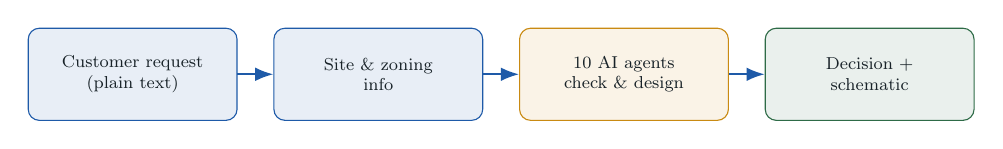
\begin{tikzpicture}[scale=0.78, every node/.style={transform shape, font=\footnotesize}]
  \foreach \i/\label/\c in {0/{Customer request\\(plain text)}/blueprint, 1/{Site \& zoning\\info}/blueprint, 2/{10 AI agents\\check \& design}/amber, 3/{Decision +\\schematic}/ok} {
    \node[draw=\c, fill=\c!10, rounded corners, minimum width=3.4cm, minimum height=1.5cm, align=center, text=ink] (n\i) at (\i*4.0,0) {\label};
  }
  \foreach \i in {0,1,2} {\pgfmathtruncatemacro{\j}{\i+1} \draw[-{Latex}, thick, blueprint] (n\i.east) -- (n\j.west);}
\end{tikzpicture}
\end{center}
\vspace{0.4cm}
\begin{itemize}
\item Agents include: parsing the request, computing the buildable envelope, matching RNGD's building-module catalog, a physics-style site simulation, and a computer-vision quality check
\item One final AI call reads everything and makes the call: approve, revise, or ``not enough information''
\end{itemize}
\end{frame}

% ---------------------------------------------------------------- 5
\begin{frame}{Pipeline: it doesn't just say yes}
\shoth{5.3cm}{hero_pipeline_decision.png}
\vspace{0.1cm}
{\small For a 120-unit request on this sample site, the AI found a real problem: the lot cannot fit the required 150 parking stalls, so it \textbf{REVISE}d the project instead of approving it --- with the exact numbers and reasons.}
\end{frame}

% ---------------------------------------------------------------- 6 section break
{%
\setbeamertemplate{footline}{}
\begin{frame}[plain]
\begin{tikzpicture}[remember picture,overlay]
  \fill[blueprintdeep] (current page.south west) rectangle (current page.north east);
\end{tikzpicture}
\begin{center}
\vspace{2.6cm}
{\color{amber}\large Now: design in real time}\\[0.4cm]
{\color{paper}\Huge\bfseries The IFC Design Studio}\\[0.6cm]
{\color{paper!70}\normalsize Move a slider. Get a real building.}
\end{center}
\end{frame}
}

% ---------------------------------------------------------------- 7
\begin{frame}{How the Design Studio works, in three steps}
\begin{columns}[T]
\column{0.32\textwidth}
\begin{block}{1. Tell it what you need}
Units, floors, unit mix, parking type, zoning preset --- a few sliders, or paste a request and let AI fill them in.
\end{block}
\column{0.32\textwidth}
\begin{block}{2. It checks the rules}
A real buildable envelope, a sample zoning code, and RNGD's \textbf{real} 2021 building-code data, all at once.
\end{block}
\column{0.32\textwidth}
\begin{block}{3. You get a real building}
A standard, open \textbf{IFC} 3D file --- the same format real architecture software uses --- instantly.
\end{block}
\end{columns}
\vspace{0.5cm}
{\small\color{muted} No AI model is required for this part --- it's fast, repeatable, rule-based engineering, so it updates the moment you move a slider.}
\end{frame}

% ---------------------------------------------------------------- 8
\begin{frame}{See it in 3D}
\shoth{5.6cm}{hero_3d.png}
\vspace{0.05cm}
{\small Every unit type, stair core, and amenity is color-coded and placed automatically from RNGD's building-module catalog --- drag to rotate, scroll to zoom, right in the browser.}
\end{frame}

% ---------------------------------------------------------------- 9
\begin{frame}{Where everything sits on the lot}
\shoth{5.6cm}{hero_siteplan.png}
\vspace{0.05cm}
{\small Blue = building, yellow = utility easement, dashed red = the buildable limit, grey = parking. This particular design only fits 23 of the 150 parking spots this program would need.}
\end{frame}

% ---------------------------------------------------------------- 10
\begin{frame}{The AI checks its own work}
\shoth{5.6cm}{hero_fail.png}
\vspace{0.05cm}
{\small Every design is scored against ten real zoning rules. Red \textbf{FAIL} rows mean exactly that --- the AI never hides a problem to make a design look good.}
\end{frame}

% ---------------------------------------------------------------- 11
\begin{frame}{Right-size the program, and it all passes}
\shoth{5.6cm}{hero_pass.png}
\vspace{0.05cm}
{\small Same tool, smaller program (60 units with podium parking instead of 120 on surface lots): \textbf{100\% match to requirements}, all ten checks pass. The Studio doesn't just flag problems --- it helps you find a design that works.}
\end{frame}

% ---------------------------------------------------------------- 12
\begin{frame}{Grounded in RNGD's own real building code}
\shoth{5.6cm}{hero_ibc.png}
\vspace{0.05cm}
{\small Not placeholder data --- RNGD's actual structured 2021 IBC rule set for their five-story hotel prototype. Here it caught something real: this corridor layout fails the real 50-ft dead-end-corridor limit, even though it passed the simpler sample check.}
\end{frame}

% ---------------------------------------------------------------- 13
\begin{frame}{It explains itself, step by step}
\shoth{5.6cm}{hero_built.png}
\vspace{0.05cm}
{\small Every design comes with a plain-language account of exactly how the numbers were computed --- not a black box.}
\end{frame}

% ---------------------------------------------------------------- 14
\begin{frame}{Ask it anything}
\begin{columns}[T]
\column{0.42\textwidth}
A chat assistant sits beside every design and always shows:
\begin{itemize}
\item A live, color-coded summary of \emph{this} design
\item A ``match to requirements'' score
\item Every setback and failed check, in plain language
\item One-click question buttons --- no typing required
\end{itemize}
\column{0.56\textwidth}
\shoth{5.9cm}{hero_chat.png}
\end{columns}
\end{frame}

% ---------------------------------------------------------------- 15 closing
{%
\setbeamertemplate{footline}{}
\begin{frame}[plain]
\begin{tikzpicture}[remember picture,overlay]
  \fill[blueprintdeep] (current page.south west) rectangle (current page.north east);
\end{tikzpicture}
\begin{center}
\vspace{1.1cm}
{\color{paper}\Large\bfseries Why this matters}\\[0.5cm]
\end{center}
\begin{columns}[T]
\column{0.32\textwidth}
\begin{center}
\color{amber}\large Speed\\[2pt]
\color{paper!80}\footnotesize Minutes, not days, for a first schematic
\end{center}
\column{0.32\textwidth}
\begin{center}
\color{amber}\large Honesty\\[2pt]
\color{paper!80}\footnotesize Flags real problems instead of hiding them
\end{center}
\column{0.32\textwidth}
\begin{center}
\color{amber}\large Grounded\\[2pt]
\color{paper!80}\footnotesize Checked against RNGD's own real code data
\end{center}
\end{columns}
\vspace{0.9cm}
\begin{center}
{\color{paper!70}\normalsize Try it:}\\[3pt]
{\color{paper}\ttfamily\small streamlit run src/app.py}\\[1cm]
{\color{paper!50}\footnotesize All zoning presets and the BaaP catalog are sample data; the IBC rules and ADA standards are RNGD's own. Prototype output --- requires licensed professional review.}
\end{center}
\end{frame}
}

\end{document}
